%%%%%%%%%%%%%%%%%%%%%%%%%%%%%%%%%%%%%%%%%%%%%%%%%%%%%%%%%%%%%%%%%%%%%%%%%%%%%%%%%%
\begin{frame}[fragile]\frametitle{}
\begin{center}
{\Large Framework}
\end{center}
\end{frame}

%%%%%%%%%%%%%%%%%%%%%%%%%%%%%%%%%%%%%%%%%%%%%%%%%%%%%%%%%%%
\begin{frame}[fragile]\frametitle{Recap: Retrieval Augmented Generation (RAG)}

\begin{center}
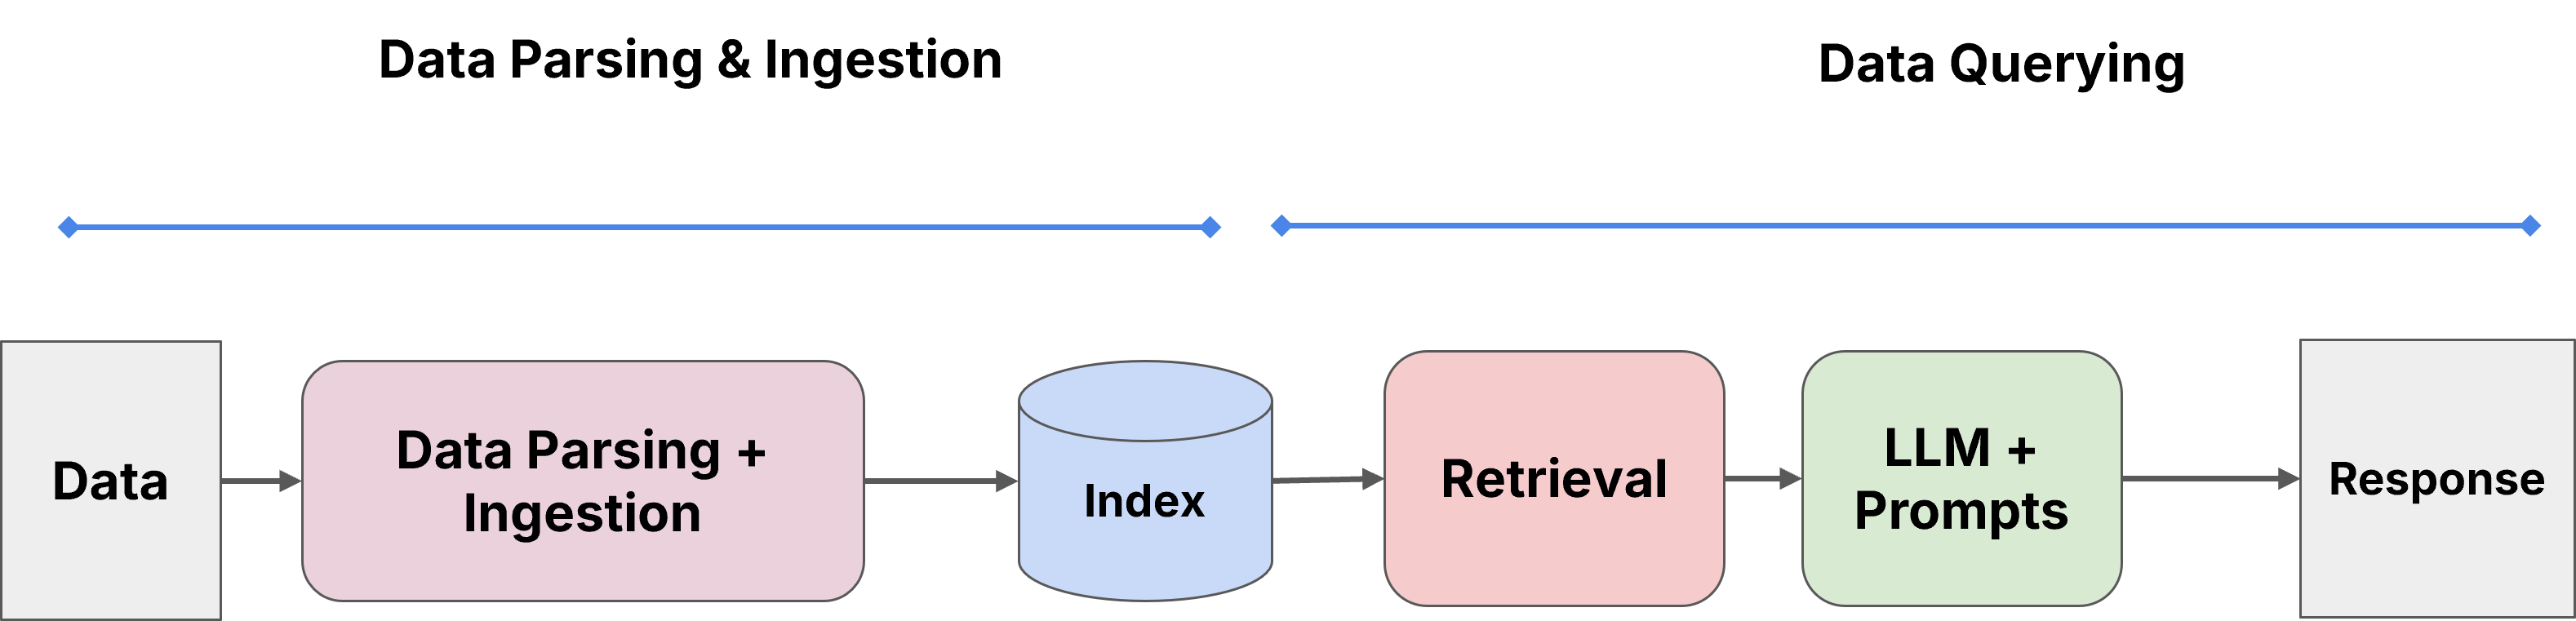
\includegraphics[width=\linewidth,keepaspectratio]{llamaindex1}

{\tiny (Ref: Data AI Summit - Databricks 2024)}
\end{center}
\end{frame}

%%%%%%%%%%%%%%%%%%%%%%%%%%%%%%%%%%%%%%%%%%%%%%%%%%%%%%%%%%%
\begin{frame}[fragile]\frametitle{Recap: Naive RAG}

\begin{center}
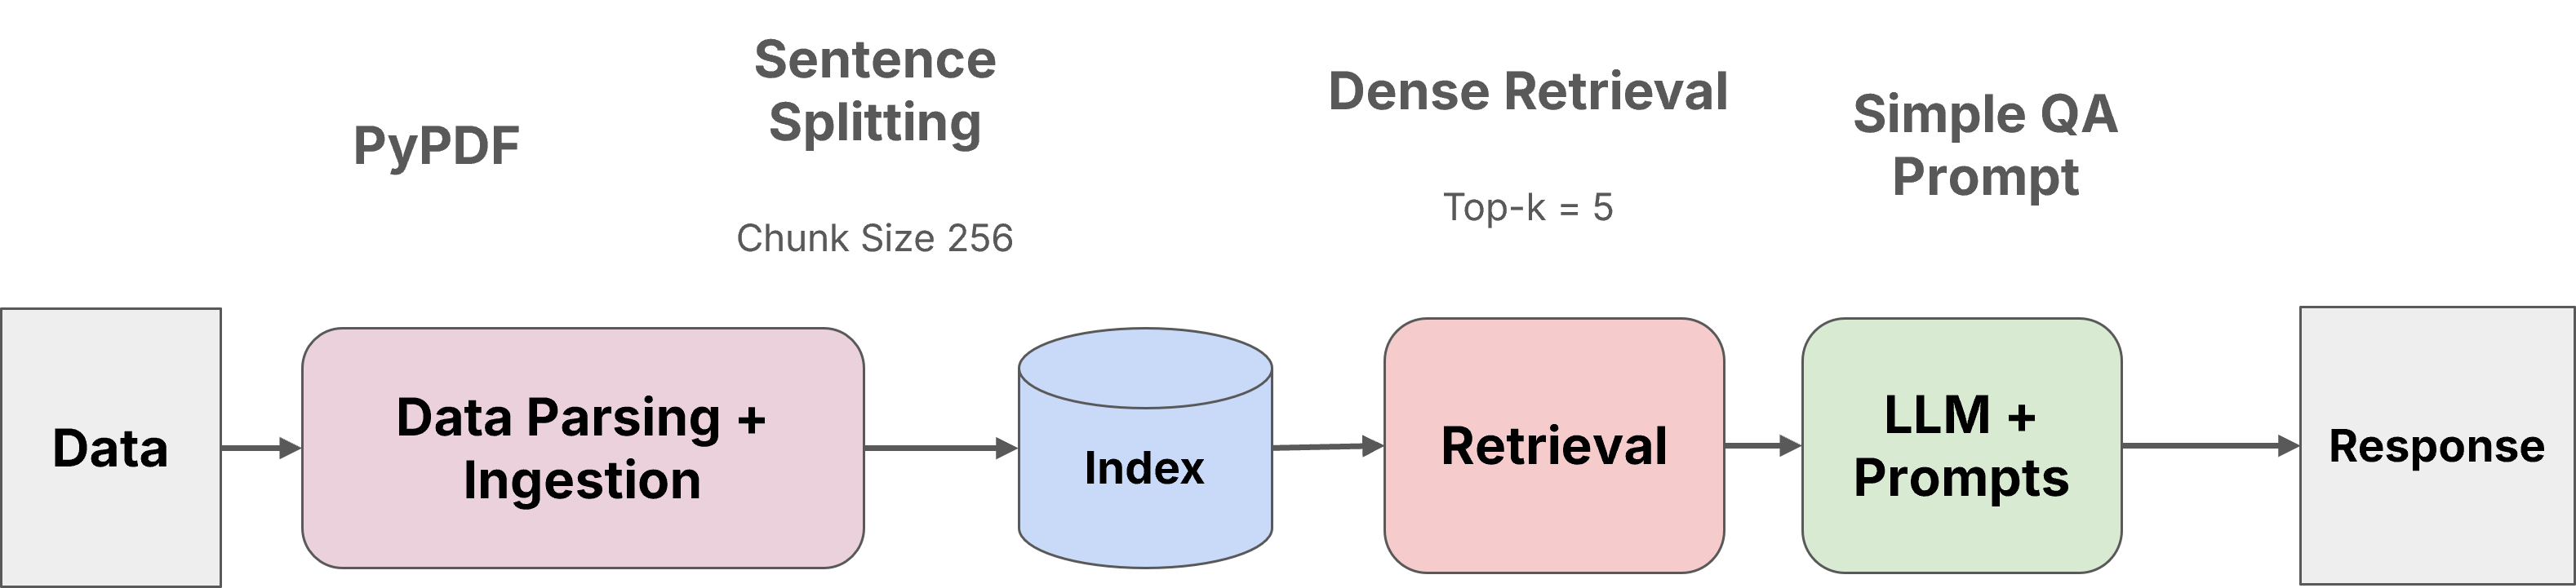
\includegraphics[width=0.8\linewidth,keepaspectratio]{llamaindex2}

{\tiny (Ref: Data AI Summit - Databricks 2024)}
\end{center}
\end{frame}


%%%%%%%%%%%%%%%%%%%%%%%%%%%%%%%%%%%%%%%%%%%%%%%%%%%%%%%%%%%
\begin{frame}[fragile]\frametitle{Challenges with Naive RAG}


\begin{itemize}
\item Easy to Prototype, Hard to Productionize
	\begin{itemize}
	\item Tend to work well for simple questions over a simple, small set of documents
	\item But productionizing RAG over more questions and a larger set of data is hard!
	\end{itemize}	
\item Failure Modes:
	\begin{itemize}
	\item Simple Questions over Complex Data
	\item Simple Questions over Multiple Documents
	\item Complex Questions 
	\end{itemize}	
\item In the naive setting, RAG is boring
	\begin{itemize}
	\item It's just a glorified search system
	\item There's many questions/tasks that naive RAG can’t give an answer to
	\item Can we build a general context-augmented research assistant?
	\end{itemize}		
\end{itemize}	

{\tiny (Ref: Data AI Summit - Databricks 2024)}

\end{frame}

%%%%%%%%%%%%%%%%%%%%%%%%%%%%%%%%%%%%%%%%%%%%%%%%%%%%%%%%%%%
\begin{frame}[fragile]\frametitle{Main Focus Areas}

\begin{center}
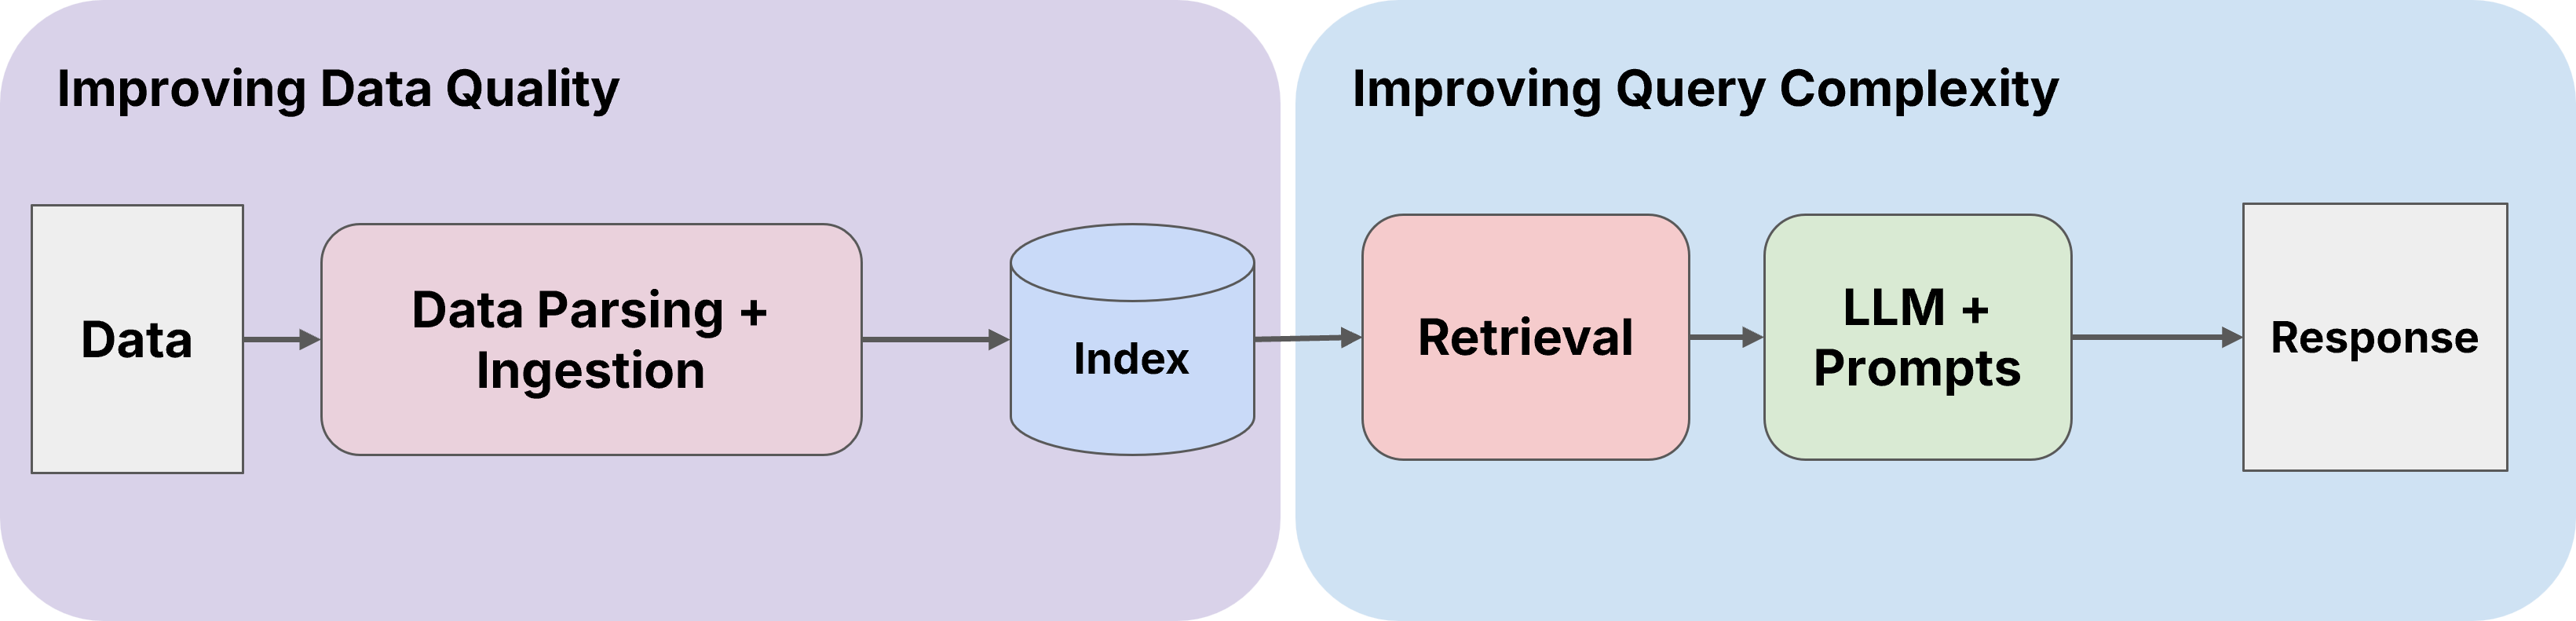
\includegraphics[width=\linewidth,keepaspectratio]{llamaindex3}

{\tiny (Ref: Data AI Summit - Databricks 2024)}
\end{center}
\end{frame}

%%%%%%%%%%%%%%%%%%%%%%%%%%%%%%%%%%%%%%%%%%%%%%%%%%%%%%%%%%%%%%%%%%%%%%%%%%%%%%%%%%
\begin{frame}[fragile]\frametitle{}
\begin{center}
{\Large Improving Data Quality}
\end{center}
\end{frame}

%%%%%%%%%%%%%%%%%%%%%%%%%%%%%%%%%%%%%%%%%%%%%%%%%%%%%%%%%%%
\begin{frame}[fragile]\frametitle{RAG is only as Good as your Data}

Garbage in $=$ Garbage Out

\begin{center}
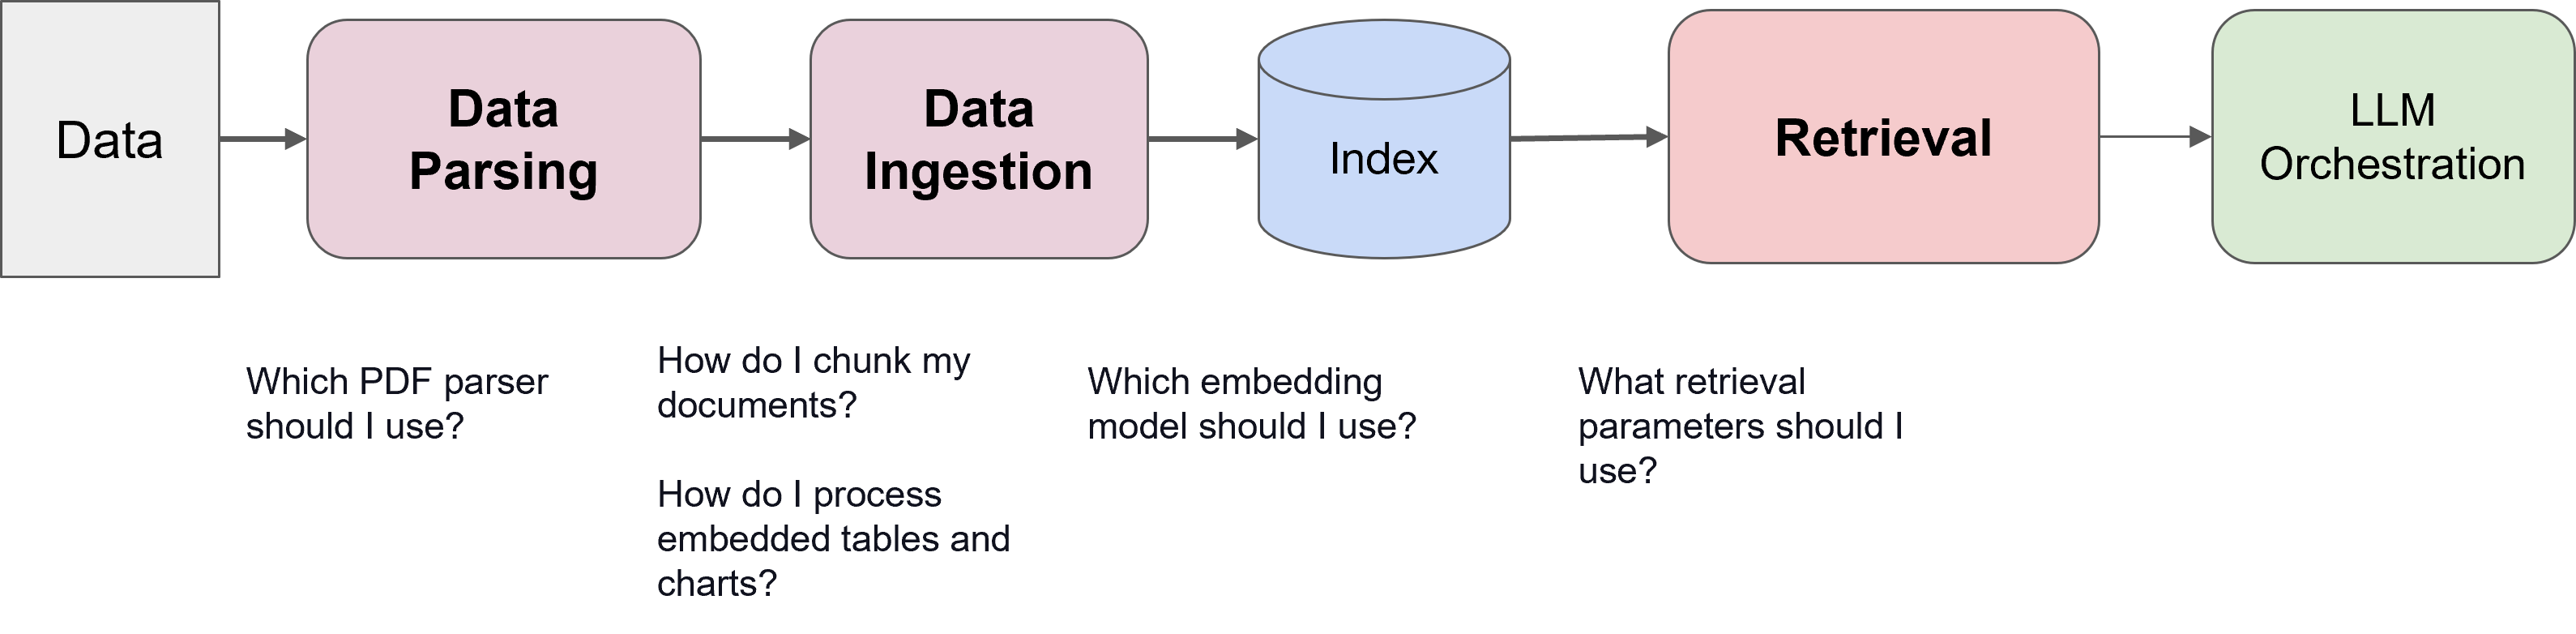
\includegraphics[width=\linewidth,keepaspectratio]{llamaindex4}

{\tiny (Ref: Data AI Summit - Databricks 2024)}
\end{center}
\end{frame}


%%%%%%%%%%%%%%%%%%%%%%%%%%%%%%%%%%%%%%%%%%%%%%%%%%%%%%%%%%%
\begin{frame}[fragile]\frametitle{RAG is only as Good as your Data}


\begin{center}
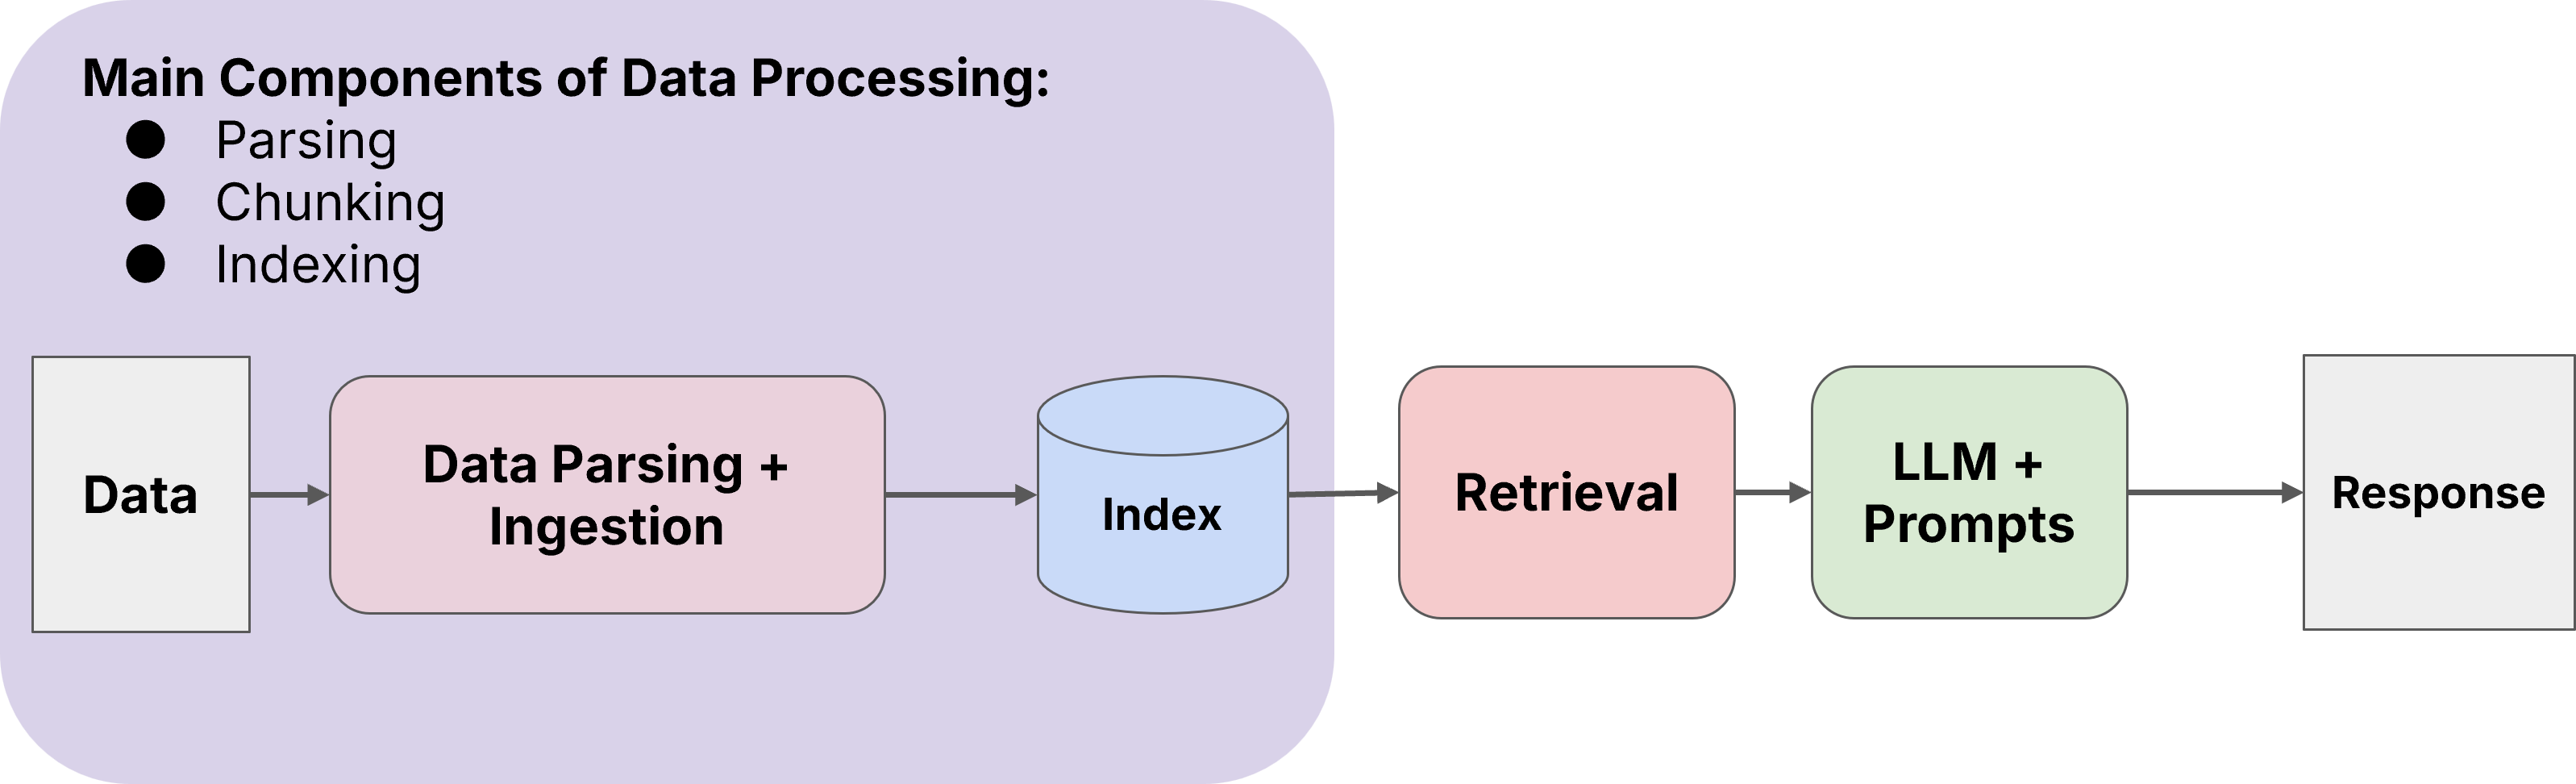
\includegraphics[width=\linewidth,keepaspectratio]{llamaindex5}

{\tiny (Ref: Data AI Summit - Databricks 2024)}
\end{center}
\end{frame}


%%%%%%%%%%%%%%%%%%%%%%%%%%%%%%%%%%%%%%%%%%%%%%%%%%%%%%%%%%%
\begin{frame}[fragile]\frametitle{General Principles}


\begin{itemize}
\item Parsing:
	\begin{itemize}
	\item Bad parsers are a key cause of garbage in == garbage out.
	\item Badly formatted text/tables confuse even the best LLMs
	\end{itemize}	
\item Chunking: 
	\begin{itemize}
	\item Try to preserve semantically similar content, say, 5 Levels of Text Splitting
	\item Strong baseline: page-level chunking
	\end{itemize}	
\item Indexing:
	\begin{itemize}
	\item Raw text often times confuses the embedding model
	\item Don’t just embed the raw text, embed references
	\item Having multiple embeddings point to the same chunk is a good practice! 
	\end{itemize}		
\end{itemize}	

{\tiny (Ref: Data AI Summit - Databricks 2024)}

\end{frame}

%%%%%%%%%%%%%%%%%%%%%%%%%%%%%%%%%%%%%%%%%%%%%%%%%%%%%%%%%%%
\begin{frame}[fragile]\frametitle{Case Study: Complex Documents}

\begin{columns}
    \begin{column}[T]{0.4\linewidth}
	A lot of documents can be classified as complex: 

		\begin{itemize}
		\item Embedded Tables, Charts, Images
		\item Irregular Layouts
		\item Headers/Footers
		\end{itemize}	
Naive RAG indexing pipelines fail over these documents.
		
    \end{column}
    \begin{column}[T]{0.6\linewidth}
		\begin{center}
		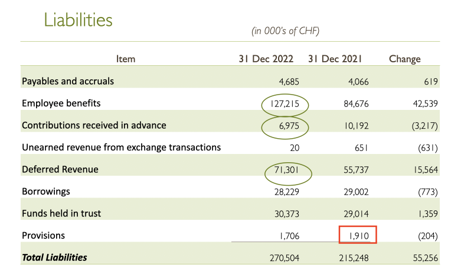
\includegraphics[width=\linewidth,keepaspectratio]{llamaindex6}

		{\tiny (Ref: Data AI Summit - Databricks 2024)}  
		\end{center}
    \end{column}
  \end{columns}
  
\end{frame}

%%%%%%%%%%%%%%%%%%%%%%%%%%%%%%%%%%%%%%%%%%%%%%%%%%%%%%%%%%%
\begin{frame}[fragile]\frametitle{Most PDF Parsing is Inadequate}
Extracts into a messy format that is impossible to pass down into more advanced ingestion/retrieval algorithms.


\begin{center}
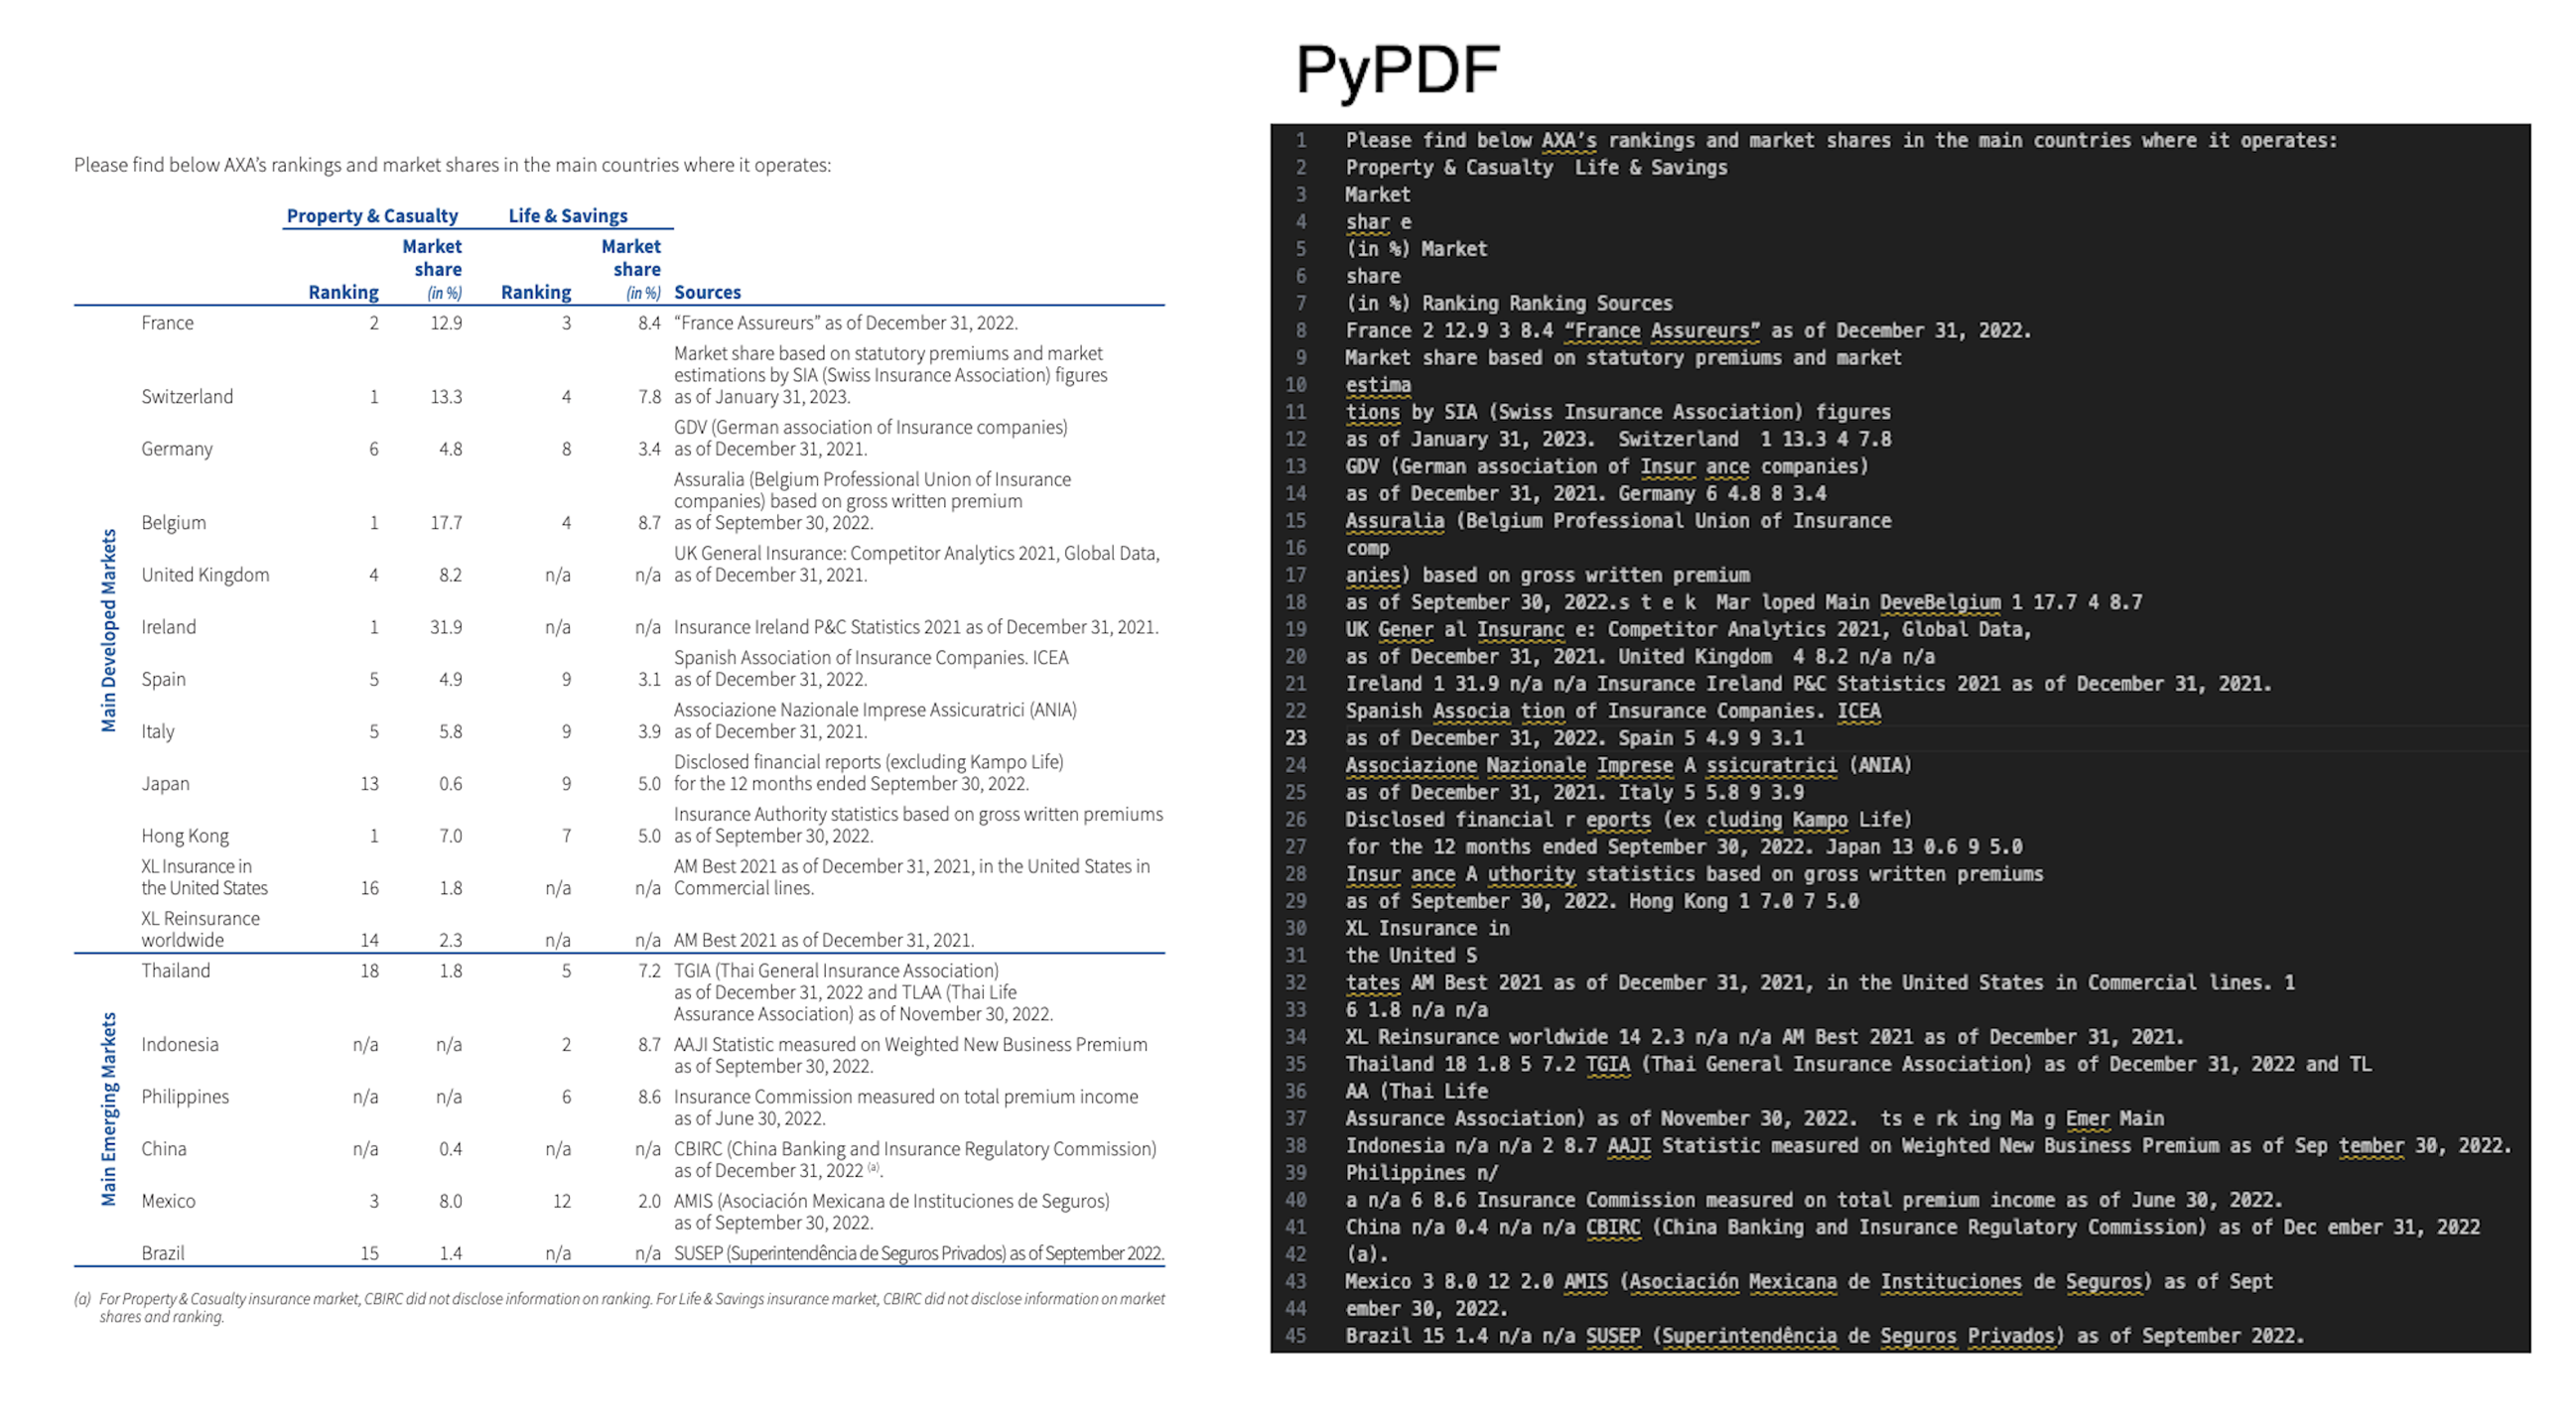
\includegraphics[width=\linewidth,keepaspectratio]{llamaindex7}

{\tiny (Ref: Data AI Summit - Databricks 2024)}
\end{center}
\end{frame}

%%%%%%%%%%%%%%%%%%%%%%%%%%%%%%%%%%%%%%%%%%%%%%%%%%%%%%%%%%%
\begin{frame}[fragile]\frametitle{LlamaParse}
A special Document Parser designed to let you build RAG over Complex docs
https://github.com/run-llama/llama\_parse


\begin{columns}
    \begin{column}[T]{0.4\linewidth}
Capabilities:
		\begin{itemize}
		\item Extracts tables / charts
		\item Input natural language parsing instructions
		\item JSON mode
		\item Image Extraction
		\item Support for more than 10 document types (.pdf, .pptx, .docx, .xml)

		\end{itemize}	
		
    \end{column}
    \begin{column}[T]{0.6\linewidth}
		\begin{center}
		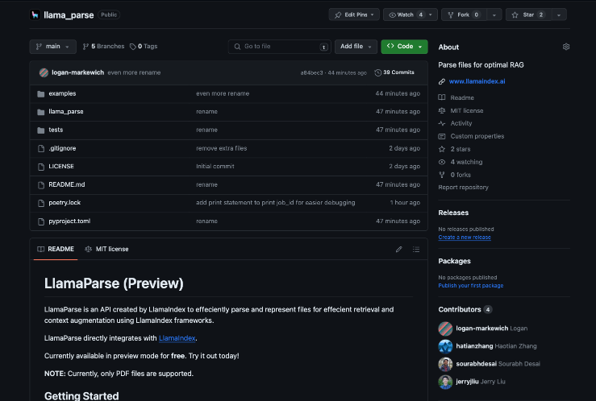
\includegraphics[width=0.8\linewidth,keepaspectratio]{llamaindex8}

		{\tiny (Ref: Data AI Summit - Databricks 2024)}
		\end{center}
    \end{column}
  \end{columns}
  
\end{frame}

%%%%%%%%%%%%%%%%%%%%%%%%%%%%%%%%%%%%%%%%%%%%%%%%%%%%%%%%%%%
\begin{frame}[fragile]\frametitle{LlamaParse $+$ Advanced Indexing}


\begin{columns}
    \begin{column}[T]{0.4\linewidth}

		\begin{itemize}
		\item Use LlamaParse to parse a document into a semi-structured markdown representation (text + tables)
		\item Use a markdown parser to extract out text and table chunks
		\item Use an LLM to extract a summary from each table → link to underlying table chunk.
		\item Index a graph of text and table chunks.
		\end{itemize}	
		
    \end{column}
    \begin{column}[T]{0.6\linewidth}
		\begin{center}
		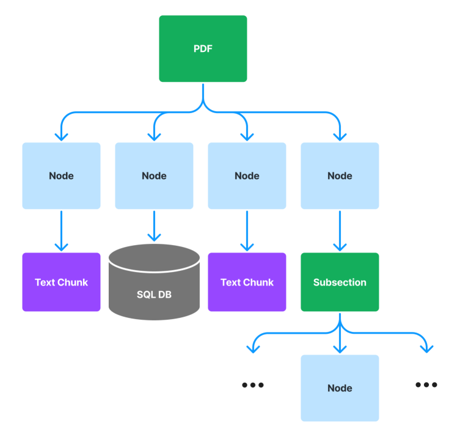
\includegraphics[width=0.8\linewidth,keepaspectratio]{llamaindex9}

		{\tiny (Ref: Data AI Summit - Databricks 2024)}
		\end{center}
    \end{column}
  \end{columns}
  


\end{frame}



%%%%%%%%%%%%%%%%%%%%%%%%%%%%%%%%%%%%%%%%%%%%%%%%%%%%%%%%%%%%%%%%%%%%%%%%%%%%%%%%%%
\begin{frame}[fragile]\frametitle{}
\begin{center}
{\Large Improving Query Complexity}
\end{center}
\end{frame}


%%%%%%%%%%%%%%%%%%%%%%%%%%%%%%%%%%%%%%%%%%%%%%%%%%%%%%%%%%%
\begin{frame}[fragile]\frametitle{Complex Questions}
There's certain questions we want to ask where naive RAG will fail.

Examples:
\begin{itemize}
\item Summarization Questions: ``Give me a summary of the entire annual report''
\item Comparison Questions: ``Compare the open-source contributions of candidate A and candidate B.''
\item Structured Analytics $+$ Semantic Search: ``Tell me about the risk factors of the highest-performing ride-share company in the US''
\item General Multi-part Questions: ``Tell me about the pro-X arguments in article A, and tell me about the pro-Y arguments in article B, make a table based on our internal style guide, then generate your own conclusion based on these facts.''
\end{itemize}	
		

 		{\tiny (Ref: Data AI Summit - Databricks 2024)}

\end{frame}

%%%%%%%%%%%%%%%%%%%%%%%%%%%%%%%%%%%%%%%%%%%%%%%%%%%%%%%%%%%
\begin{frame}[fragile]\frametitle{Query Planning}

\begin{itemize}
\item Break down query into parallelizable sub-queries.
\item Each can be execute-query-ed against any set of RAG pipelines
\item Example: Compare revenue of Uber and Lyft in 2021
\end{itemize}	

\begin{center}
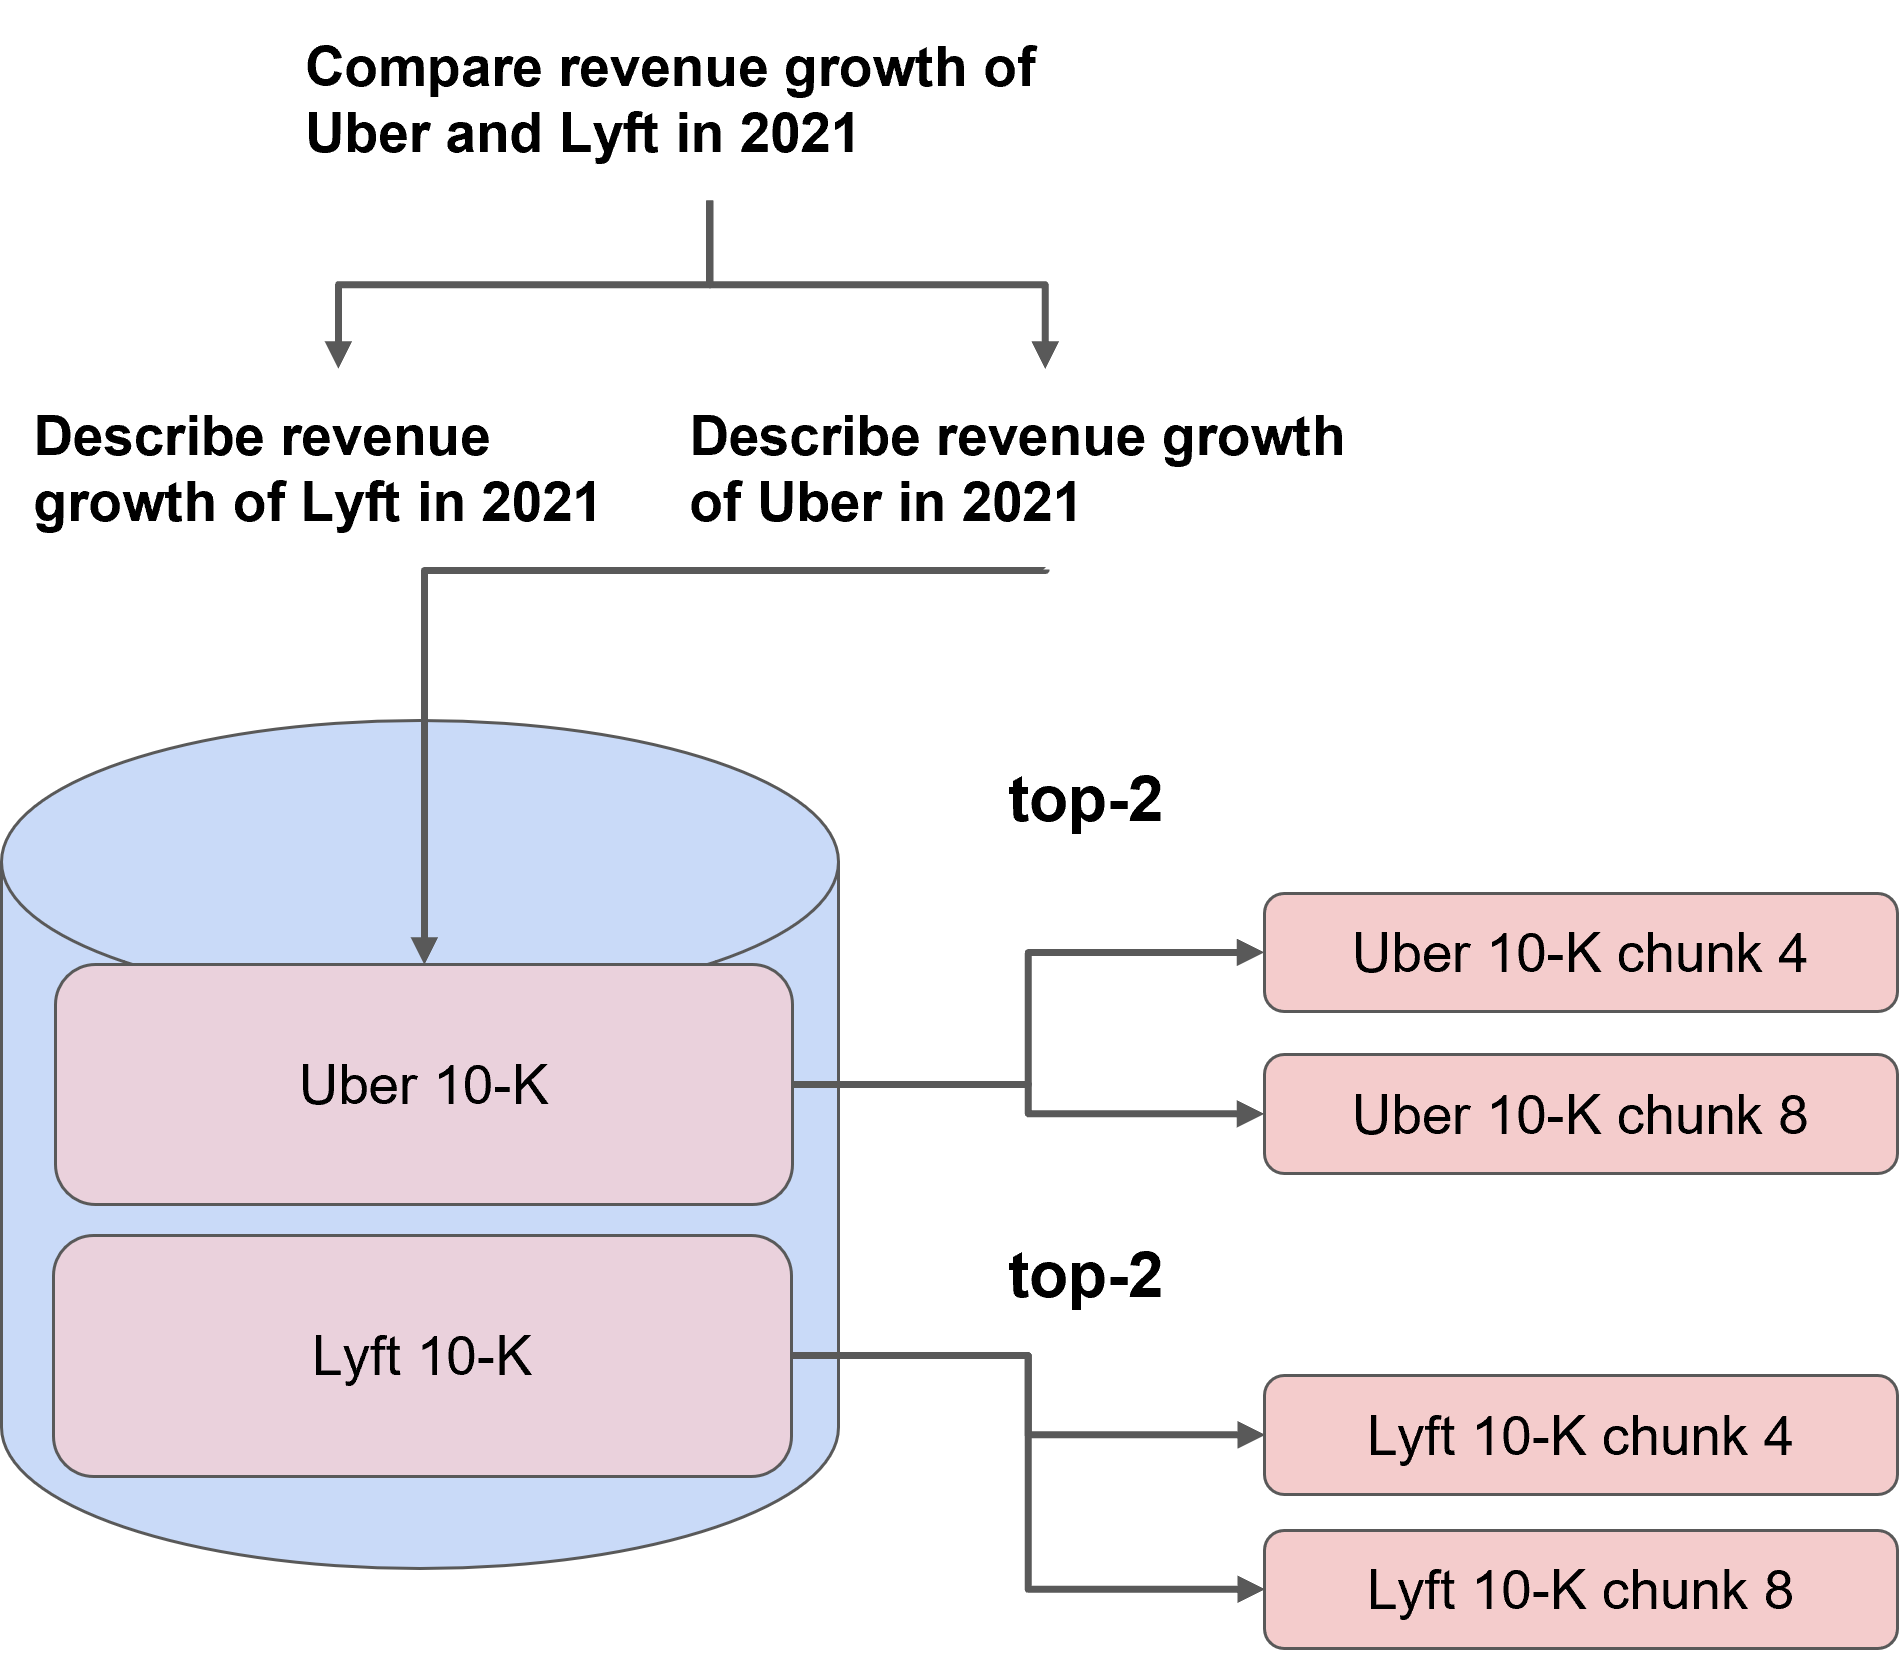
\includegraphics[width=0.5\linewidth,keepaspectratio]{llamaindex10}

{\tiny (Ref: Data AI Summit - Databricks 2024)}
\end{center}
\end{frame}

% %%%%%%%%%%%%%%%%%%%%%%%%%%%%%%%%%%%%%%%%%%%%%%%%%%%%%%%%%%%
% \begin{frame}[fragile]\frametitle{Tool Use}

% \begin{columns}
    % \begin{column}[T]{0.4\linewidth}

		% \begin{itemize}
		% \item Use an LLM to call an API
		% \item Infer the parameters of that API
		% \item In normal RAG you just pass through the query.
		% \item But what if you used the LLM to infer all the parameters for the API interface?
		% \item A key capability in many QA use cases (auto-retrieval, text-to-SQL, and more)
		% \end{itemize}	
		
    % \end{column}
    % \begin{column}[T]{0.6\linewidth}
		% \begin{center}
		% 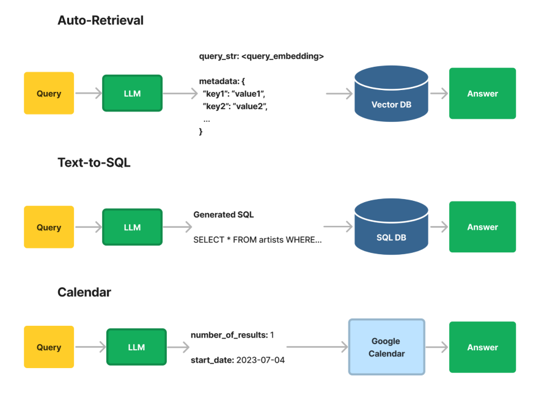
\includegraphics[width=0.8\linewidth,keepaspectratio]{llamaindex11}

		% {\tiny (Ref: Data AI Summit - Databricks 2024)}
		% \end{center}
    % \end{column}
  % \end{columns}

% \end{frame}

%%%%%%%%%%%%%%%%%%%%%%%%%%%%%%%%%%%%%%%%%%%%%%%%%%%%%%%%%%%%%%%%%%%%%%%%%%%%%%%%%%
\begin{frame}[fragile]\frametitle{}
\begin{center}
{\Large Concepts}
\end{center}
\end{frame}



%%%%%%%%%%%%%%%%%%%%%%%%%%%%%%%%%%%%%%%%%%%%%%%%%%%%%%%%%%%
\begin{frame}[fragile]\frametitle{Work-flow}

\begin{center}
\includegraphics[width=\linewidth,keepaspectratio]{llm18}

{\tiny (Ref: LlamaIndex: A Central Interface between LLM's + your external data)}
\end{center}
\end{frame}



%%%%%%%%%%%%%%%%%%%%%%%%%%%%%%%%%%%%%%%%%%%%%%%%%%%%%%%%%%%
\begin{frame}[fragile]\frametitle{Data Connectors: powered by LlamaHub}


\begin{itemize}
\item Easily ingest any kind of data, from anywhere, into unified document containers 
\item Powered by community-driven hub, rapidly growing (90+ loaders and counting!)
\item Growing support for multimodal documents (e.g. with inline images)
\end{itemize}	

$<10$ lines of code to ingest from Notion

\begin{center}
\includegraphics[width=0.8\linewidth,keepaspectratio]{llm16}

{\tiny (Ref: LlamaIndex: A Central Interface between LLM's + your external data)}
\end{center}
\end{frame}

%%%%%%%%%%%%%%%%%%%%%%%%%%%%%%%%%%%%%%%%%%%%%%%%%%%%%%%%%%%
\begin{frame}[fragile]\frametitle{Data Indices + Query Interface}


\begin{itemize}
\item Source documents are stored in a data collection, In-memory, MongoDB
\item Data indices help to provide a view of your raw data, Vectors, keyword lookups, summaries
\item A retriever helps to retrieve relevant documents for your query
\item A query engine manages retrieval and synthesis given the query. 
\end{itemize}	

\begin{center}
\includegraphics[width=0.6\linewidth,keepaspectratio]{llm17}

{\tiny (Ref: LlamaIndex: A Central Interface between LLM's + your external data)}
\end{center}

\end{frame}

%%%%%%%%%%%%%%%%%%%%%%%%%%%%%%%%%%%%%%%%%%%%%%%%%%%%%%%%%%%
\begin{frame}[fragile]\frametitle{Data Ingestion: LlamaHub}


\begin{center}
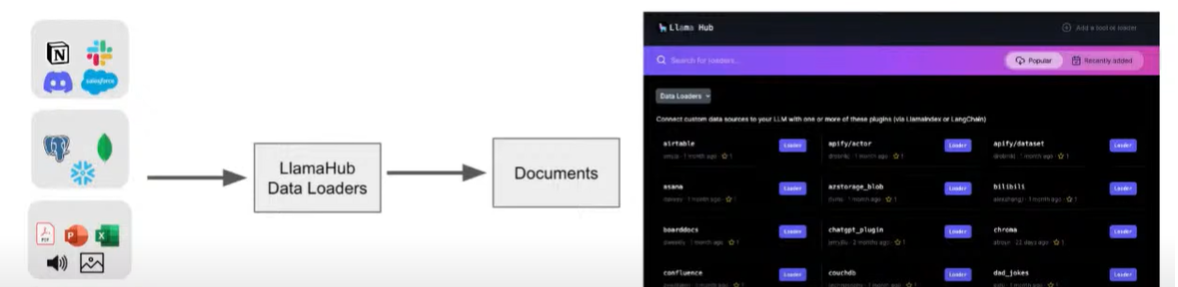
\includegraphics[width=\linewidth,keepaspectratio]{llamaindex12}

{\tiny (Ref: Getting started with LlamaIndex - AI Planet)}
\end{center}
\end{frame}


%%%%%%%%%%%%%%%%%%%%%%%%%%%%%%%%%%%%%%%%%%%%%%%%%%%%%%%%%%%
\begin{frame}[fragile]\frametitle{Data Indexing}

\begin{itemize}
\item Documents are split ie chunking and embedding for each chunk is created
\item Chunk $+$ Embedding is capsuled as 'Node'.
\item All Nodes are stored in 'in-memory index' or Vector Db (e.g. PineCone, Weaviate, Qdrant)
\end{itemize}	

\begin{center}
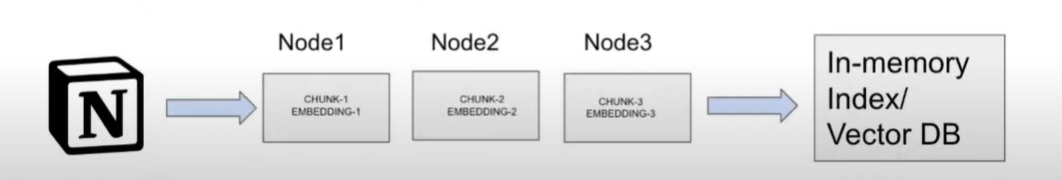
\includegraphics[width=\linewidth,keepaspectratio]{llamaindex13}

{\tiny (Ref: Getting started with LlamaIndex - AI Planet)}
\end{center}
\end{frame}



%%%%%%%%%%%%%%%%%%%%%%%%%%%%%%%%%%%%%%%%%%%%%%%%%%%%%%%%%%%
\begin{frame}[fragile]\frametitle{Vector Store Index}

Nodes are stored in Vector Db, where each node has chunk $+$ embedding.

\begin{center}
\includegraphics[width=0.8\linewidth,keepaspectratio]{llm19}

{\tiny (Ref: LlamaIndex: A Central Interface between LLM's + your external data)}
\end{center}
\end{frame}

%%%%%%%%%%%%%%%%%%%%%%%%%%%%%%%%%%%%%%%%%%%%%%%%%%%%%%%%%%%
\begin{frame}[fragile]\frametitle{Retrieval}

When User asks a query:
\begin{itemize}
\item It retrieves the relevant nodes, ranks them based on the embedding similarity between query and nodes.
\item Post processes the retrieved nodes if needed.
\item Directs the processed nodes to Response Synthesis module.
\end{itemize}	



\begin{center}
\includegraphics[width=0.6\linewidth,keepaspectratio]{llm20}

{\tiny (Ref: LlamaIndex: A Central Interface between LLM's + your external data)}
\end{center}
\end{frame}

%%%%%%%%%%%%%%%%%%%%%%%%%%%%%%%%%%%%%%%%%%%%%%%%%%%%%%%%%%%
\begin{frame}[fragile]\frametitle{Response Synthesis}

Collect answers from all, then collate and then send to final answer.

\begin{center}
\includegraphics[width=\linewidth,keepaspectratio]{llm21}

{\tiny (Ref: LlamaIndex: A Central Interface between LLM's + your external data)}
\end{center}
\end{frame}

%%%%%%%%%%%%%%%%%%%%%%%%%%%%%%%%%%%%%%%%%%%%%%%%%%%%%%%%%%%
\begin{frame}[fragile]\frametitle{Response Synthesis}

Collect answers one after another and then send to final answer.

\begin{center}
\includegraphics[width=\linewidth,keepaspectratio]{llm22}

{\tiny (Ref: LlamaIndex: A Central Interface between LLM's + your external data)}
\end{center}
\end{frame}


% %%%%%%%%%%%%%%%%%%%%%%%%%%%%%%%%%%%%%%%%%%%%%%%%%%%%%%%%%%%
% \begin{frame}[fragile]\frametitle{Response Synthesis}

% Given a query, get answer from Node 1, generate intermediate answer, then with at plus Node2 info, generate step by step till final answer.


% \begin{center}
% 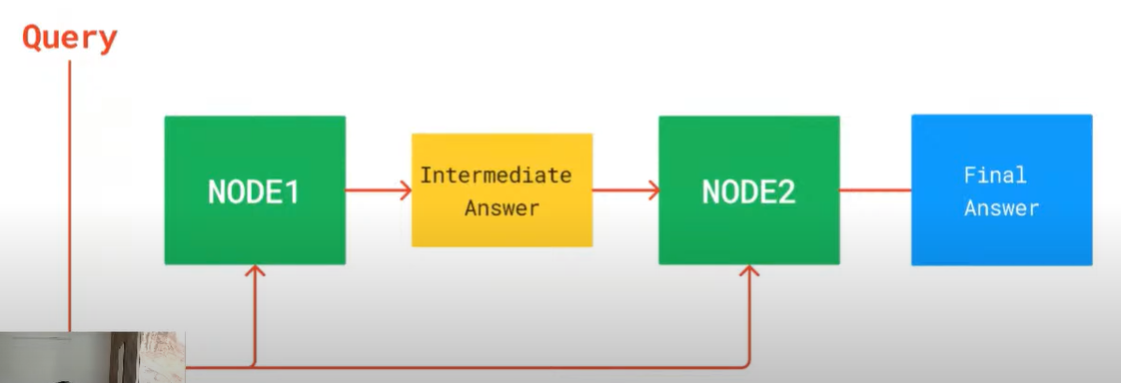
\includegraphics[width=\linewidth,keepaspectratio]{llamaindex14}

% {\tiny (Ref: LlamaIndex: A Central Interface between LLM's + your external data)}
% \end{center}
% \end{frame}


%%%%%%%%%%%%%%%%%%%%%%%%%%%%%%%%%%%%%%%%%%%%%%%%%%%%%%%%%%%
\begin{frame}[fragile]\frametitle{Response Synthesis}

\begin{center}
\includegraphics[width=\linewidth,keepaspectratio]{llm23}

{\tiny (Ref: LlamaIndex: A Central Interface between LLM's + your external data)}
\end{center}
\end{frame}

%%%%%%%%%%%%%%%%%%%%%%%%%%%%%%%%%%%%%%%%%%%%%%%%%%%%%%%%%%%
\begin{frame}[fragile]\frametitle{Response Synthesis}

\begin{center}
\includegraphics[width=0.6\linewidth,keepaspectratio]{llm24}

{\tiny (Ref: LlamaIndex: A Central Interface between LLM's + your external data)}
\end{center}
\end{frame}

%%%%%%%%%%%%%%%%%%%%%%%%%%%%%%%%%%%%%%%%%%%%%%%%%%%%%%%%%%%
\begin{frame}[fragile]\frametitle{Multi level Queries}

\begin{center}
\includegraphics[width=0.6\linewidth,keepaspectratio]{llm25}

{\tiny (Ref: LlamaIndex: A Central Interface between LLM's + your external data)}
\end{center}
\end{frame}

%%%%%%%%%%%%%%%%%%%%%%%%%%%%%%%%%%%%%%%%%%%%%%%%%%%%%%%%%%%
\begin{frame}[fragile]\frametitle{Multi level Queries}

\begin{center}
\includegraphics[width=\linewidth,keepaspectratio]{llm26}

{\tiny (Ref: LlamaIndex: A Central Interface between LLM's + your external data)}
\end{center}
\end{frame}

%%%%%%%%%%%%%%%%%%%%%%%%%%%%%%%%%%%%%%%%%%%%%%%%%%%%%%%%%%%
\begin{frame}[fragile]\frametitle{Multi level Queries}

\begin{center}
\includegraphics[width=\linewidth,keepaspectratio]{llm27}

{\tiny (Ref: LlamaIndex: A Central Interface between LLM's + your external data)}
\end{center}
\end{frame}